\chapter{Contexte}
\section{L'entreprise : Aboard Engineering}
Aboard Engineering est un bureau d'études en automatique, électronique et informatique industrielle. Composé d'experts en contrôle et instrumentation de systèmes embarqués temps réel, ses ingénieurs développent des solutions pour des applications civiles et militaires. De la R\&D à la série, Aboard Engineering travail dans le domaine des transports (automobile, aéronotique, marin), de l'off-road (agriculture, engins de chantier, ...) et de l'industrie. Les figures \ref{fig:domaines} et  \ref{fig:metiers} sont tirées du site web d'Aboard Engineering et récapitulent les domaines et métiers de la société.

\begin{figure}[h]
	\center
	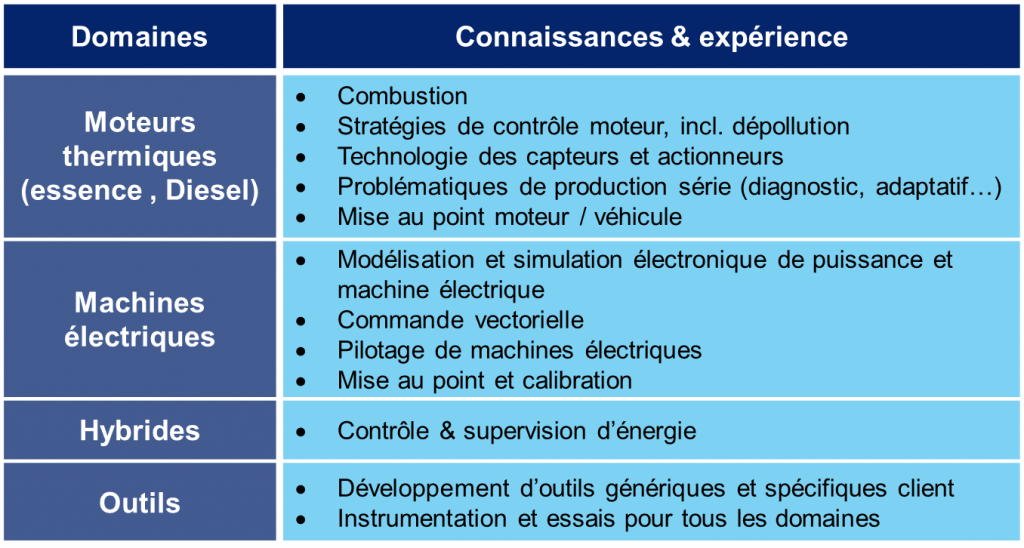
\includegraphics[scale=0.4]{images/domaines}
	\caption{Domaines -- Source : Abord Engineering}
	\label{fig:domaines}
\end{figure}

\begin{figure}[h]
	\center
	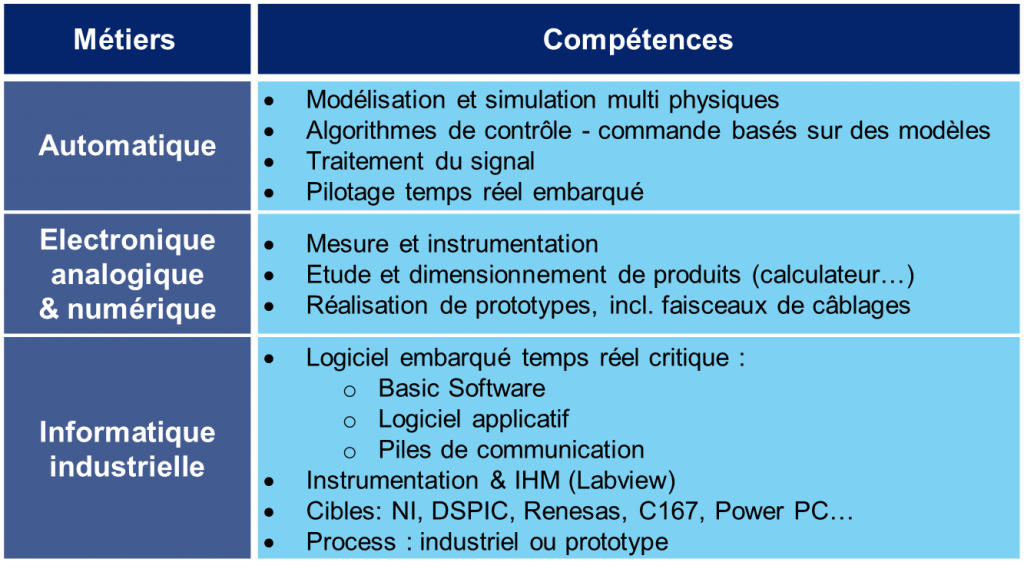
\includegraphics[scale=0.4]{images/metiers}
	\caption{Métiers et Compétences -- Source : Abord Engineering}
	\label{fig:metiers}
\end{figure}

\section{La plateforme Orianne}
\label{sec:orianne}

Aboard Engineering fournie différents types de produits et services. Je ne vais ici développer que le cas de la plateforme \gloss{orianne} sur laquelle j'ai travaillé.

\gloss{orianne} est une plateforme de prototypage rapide de fonctions de contrôle moteurs.
Elle permet de regrouper différents modules d'un calculateur moteurs (transmission, ABS, injection, couple moteur, etc.) afin de générer une unique application qui sera déployée dans un calculateur moteur.
Pour cela, une interface graphique permet de configurer quelles fonctions sont à intégrer dans l'application (elles-mêmes configurables), les caractéristiques du moteur cible, la configuration du \gloss{rtos} (définition des récurrence des tâches).
Une fois l'application configurée, la plateforme va chercher les codes sources des modules sélectionnés, génère les fichiers sources manquant (non relatifs à des fonctions moteurs) et  effectue la compilation.
La sortie produite est un fichier binaire représentant le code source compilé ainsi qu'un fichier \og dictionnaire \fg{} associant chaque élément à l'adresse à laquelle il sera stocké dans la mémoire du calculateur. Ce fichier contient les adresses des constantes, des calibrations, des différentes fonctions appelées, etc. Les données non modifiées durant l'exécution de l'application.
L'intérêt d'avoir des adresses fixes et connues pour ces éléments est qu'il est possible via un logiciel tiers de récupérer ces informations et de les modifiées directement dans la mémoire sans avoir à déployer une nouvelle application. Pour rappel, nous sommes dans un cadre R\&D et beaucoup de tests sont effectués sur banc de test et le besoin d'adapter les calibrations pour obtenir le meilleur comportement est primordial.

La plateforme en elle-même est composée de plusieurs outils :
\begin{itemize}
	\item Configuration du moteur cible
	\item Configuration des fonctions moteur
	\item Configuration du \gloss{rtos}
	\item Générations des fichiers sources
	\item Compilation de l'application
\end{itemize}

\section{L'environnement de travail //TODO}
\lipsum
